\pgfmathsetmacro\nava{0}
\chapter{Avaliação Arquitetural ATAM}

A avaliação arquitetural ATAM (Architecture Tradeoff Analysis Method) tem como objetivo elicitar e refinar os requisitos de atributos de qualidade e 
as decisões de arquitetura no projeto de software.\cite{Mendes:2002}

\section{Análise das abordagens arquiteturais}
\vspace{0.5cm}

Abaixo listamos as abordagens arquiteturais, seus cenários, importância e complexidade(definidas em B - baixa, M - média e A - Alta).

\vspace{0.5cm}

\pgfmathtruncatemacro\nava{\nava + 1}
\subsection{Manutenabilidade}
Cenário \nava: A arquitetura deve considerar a facilidade de manutenção do sistema ao longo do tempo, buscando
criar uma estrutura que permita a evolução do sistema, isto pode ser atingido utilizando de padrões de projetos. 
Por exemplo na utilização do padrão MVC, separação das responsabilidades.

\vspace{0.5cm}
\noindent\textbf{\textit{Importância:}} \textit{A -} \textbf{\textit{Complexidade:}} \textit{A}
\vspace{0.5cm}

\pgfmathtruncatemacro\nava{\nava + 1}
\subsection{Usabilidade}
Cenário \nava: A arquitetura deve considerar a usabilidade do sistema, facilitando a utilização do mesmo por parte dos usuários,
além de permitir uma fácil integração de novos usuários ao sistema. Para isto deve se adotar padrões de interface, tanto em dispositivos
móveis como em telas maiores como monitores, utilizar de interfaces intuitivas e que o padrão seja mantido entre as telas do sistema.

\vspace{0.5cm}
\noindent\textbf{\textit{Importância:}} \textit{A -} \textbf{\textit{Complexidade:}} \textit{M}
\vspace{0.5cm}

\pgfmathtruncatemacro\nava{\nava + 1}
\subsection{Segurança}
Cenário \nava: A arquitetura deve ser pensada em tornar as informações protegidas e garantir acesso seguro ao sistema.
Um usuário não autorizado não deve conseguir acessar informações confidênciais do sistema. Para isso pdoe se adotar 
criptografia nas senhas e controle de autenticação e autorização no sistema.

\vspace{0.5cm}
\noindent\textbf{\textit{Importância:}} \textit{A -} \textbf{\textit{Complexidade:}} \textit{A}
\vspace{0.5cm}

\pgfmathtruncatemacro\nava{\nava + 1}
\subsection{Interoperabilidade}
Cenário \nava: A arquitetura deve considerar a capacidade do sistema em se comunicar com outros sistemas de software
em outras tecnologias, para isso deve-se adotar padrões de comunicação que são amplamente aceitos como RESTFUL, SOAP
e na utilização de formatos de dados amplamente utilizados como JSON e XML.

\vspace{0.5cm}
\noindent\textbf{\textit{Importância:}} \textit{A -} \textbf{\textit{Complexidade:}} \textit{M}
\vspace{0.5cm}

\pgfmathtruncatemacro\nava{\nava + 1}
\subsection{Desempenho}
Cenário \nava: A arquitetura deve considerar a capacidade do sistema em se manter estável e atingir requisitos de 
tempo de respostas quando de alta carga de trabalho, como horários de pico. Para isso a arquitetura deve ser pensada de modo 
a oferecer o dimensionamento de recursos, seja horizontal ou vertical e caches para informações estáticas.

\vspace{0.5cm}
\noindent\textbf{\textit{Importância:}} \textit{M -} \textbf{\textit{Complexidade:}} \textit{A}
\vspace{0.5cm}

\pgfmathsetmacro\cen{0}
\section{Cenários}
\vspace{0.5cm}

Abaixo listamos os cenários para serem efetuados testes na aplicação, os mesmos demonstram como serão satisfeitos os 
atributos de qualidade do software(requisitos não funcionais).

\pgfmathtruncatemacro\cen{\cen + 1}
\subsection{Cenário \cen} 
Manutenabilidade: Quando da necessidade de se atualizar um requisito de negócio do sistema, é necessário a modificação
em alguma camada do mesmo, portanto é fundamental o software ser desenvolvido em camadas e com baixo acoplamento 
entre as mesmas, permitindo assim uma fácil manutenção e evolução do software. O atendimento deste cenário atende o 
RNF-1 - Desenvolvimento em Camadas.

\pgfmathtruncatemacro\cen{\cen + 1}
\subsection{Cenário \cen} 
Usabilidade: Ao acessar o software de diferentes dispositivos o sistema deverá se adaptar ao tamanho das telas, além de 
ter um padrão visual entre telas e dispositivos de modo a facilitar o aprendizado do mesmo. O atendimento deste cenário 
atende o RNF-2 - Padrão de Interface.

\pgfmathtruncatemacro\cen{\cen + 1}
\subsection{Cenário \cen} 
Segurança: O sistema deverá criptografar dados sensivés do software, como a senha de acesso do usuário. O atendimento deste cenário 
atende o RNF-3 - Banco de dados.

\pgfmathtruncatemacro\cen{\cen + 1}
\subsection{Cenário \cen} 
Segurança: Ao tentar acessar um recurso privado sem estar logado o sistema deverá exibir uma mensagem de não autorizado. O atendimento deste cenário 
atende o RNF-4 - Autenticação/Autorização.

\pgfmathtruncatemacro\cen{\cen + 1}
\subsection{Cenário \cen} 
Interoperabilidade: Ao efetuar um pagamento através do software, o sistema deverá realizar uma comunicação com algum meio de pagamento para permitir a cobrança do cliente. O atendimento deste cenário 
atende o RNF-5 - Comunicação com sistema de pagamento.


\pgfmathtruncatemacro\cen{\cen + 1}
\subsection{Cenário \cen} 
Desempenho: Ao efetuar login no sistema, o mesmo deverá validar e permitir ou negar o acesso em até 5 segundos, permitindo assim uma
experiência fluida para o usuário. O atendimento deste cenário atende o RNF-6 - Acesso após Autenticação.

\pgfmathsetmacro\avcen{0}
\section{Evidências da Avaliação de Cenários}
\vspace{0.5cm}


\pgfmathtruncatemacro\avcen{\avcen + 1}
\subsection{Cenário \avcen} 
\noindent
\begin{tabular}{|>{\raggedright\arraybackslash}p{3cm}|>{\raggedright\arraybackslash}p{10cm}|}
    \hline
    \cellcolor[gray]{0.8}Atributo de Qualidade & Manutenabilidade \\
    \hline
    \cellcolor[gray]{0.8}Requisito de Qualidade & A arquitetura deve considerar a facilidade de manutenção do sistema ao longo do tempo, buscando criar uma estrutura que permita a evolução do sistema. \\
    \hline
    \multicolumn{2}{|l|}{\cellcolor[gray]{0.8}Preocupação:} \\
    \hline
    \multicolumn{2}{|p{13cm}|}{O sistema deverá ser feito utilizando padrão MVC, sendo assim desenvolvido em camadas de modo a facilitar a manutenabilidade do mesmo.} \\
    \hline
    \multicolumn{2}{|l|}{\cellcolor[gray]{0.8}Cenário(s):} \\
    \hline
    \multicolumn{2}{|p{13cm}|}{Cenário \avcen} \\
    \hline 
    \multicolumn{2}{|l|}{\cellcolor[gray]{0.8}Ambiente:} \\
    \hline        
    \multicolumn{2}{|p{13cm}|}{Operação normal} \\
    \hline     
    \multicolumn{2}{|l|}{\cellcolor[gray]{0.8}Estímulo:} \\
    \hline  
    \multicolumn{2}{|p{13cm}|}{Ao sofrer uma mudança de requisitos, como adição de novos campos.} \\    
    \hline     
    \multicolumn{2}{|l|}{\cellcolor[gray]{0.8}Mecanismo} \\
    \hline  
    \multicolumn{2}{|p{13cm}|}{Utilização de classes seguindo o modelo MVC e boas práticas de codificação de modo a separar as responsabilidades de cada classe} \\
    \hline 
    \multicolumn{2}{|l|}{\cellcolor[gray]{0.8}Medida de Resposta} \\
    \hline            
    \multicolumn{2}{|p{13cm}|}{Tempo gasto e facilidade para implementar mudanças de requisito} \\
    \hline 
    \multicolumn{2}{|l|}{\cellcolor[gray]{0.8}Considreação sobre a arquitetura:} \\
    \hline  
    \cellcolor[gray]{0.8}Riscos &  A adoção do padrão MVC pode resultar em uma arquitetura inicial mais complexa, exigindo uma correta implementação no decorrer do desenvolvimento.\\
    \hline           
    \cellcolor[gray]{0.8}Pontos de Sensibilidade &  Caso o sistema seja frequentemente alterado poderá vir a ser necessário uma revisão mais próxima e constante na estrutura da arquitetura para continuar garantindo a manutenabilidade.\\
    \hline           
    \cellcolor[gray]{0.8}Tradeoff &  No inicio do desenvolvimento poderá ocorrer um aumento na complexidade, o que será recompensado pela facilidade de manutenção a longo prazo.\\
    \hline         
\end{tabular}

\subsubsection{Evidência do Cenário \avcen} 

O desenvolvimento é no padrão arquitetural MVC, para isso utilizamos a separação das classes seguindo as regras do padrão, colocando
uma camada de controller para direcionar o fluxo, uma camada de modelo para representar as tabelas do banco, para isso utilizamos também o 
padrão repository e uma camada de serviço que contém as regras de negócio.

\begin{figure}[h]
   \centering
   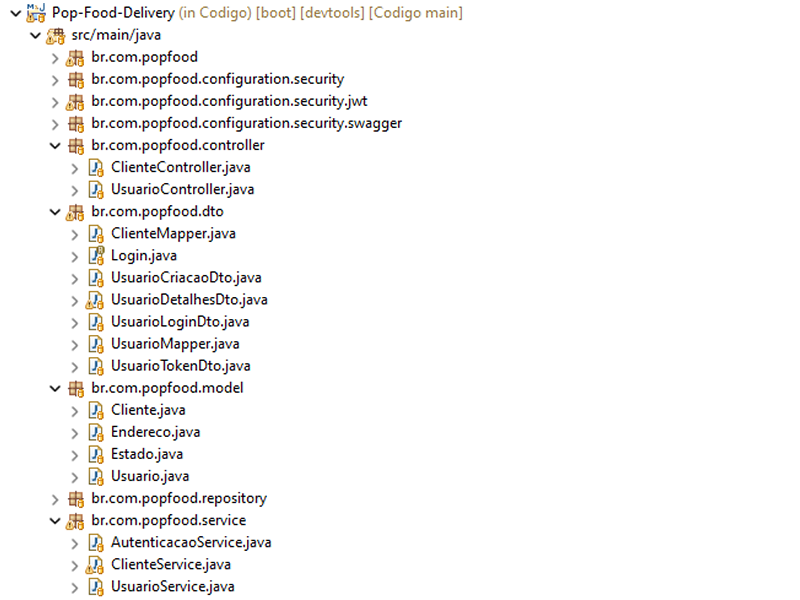
\includegraphics[width=1\textwidth]{padrao_mvc.png}
   \caption{Padrão MVC}
   \label{fig:Padrao MVC}
\end{figure}

\pgfmathtruncatemacro\avcen{\avcen + 1}
\subsection{Cenário \avcen} 
\noindent
\begin{tabular}{|>{\raggedright\arraybackslash}p{3cm}|>{\raggedright\arraybackslash}p{10cm}|}
    \hline
    \cellcolor[gray]{0.8}Atributo de Qualidade & Usabilidade \\
    \hline
    \cellcolor[gray]{0.8}Requisito de Qualidade & O software deve ter uma boa usabilidade mantendo o padrão e a adaptabilidade em diferentes telas. \\
    \hline
    \multicolumn{2}{|l|}{\cellcolor[gray]{0.8}Preocupação:} \\
    \hline
    \multicolumn{2}{|p{13cm}|}{Ao ser acessado de diferentes dispositivos o padrão deverá ser mantido e adaptado a resoluções diferentes.} \\
    \hline
    \multicolumn{2}{|l|}{\cellcolor[gray]{0.8}Cenário(s):} \\
    \hline
    \multicolumn{2}{|p{13cm}|}{Cenário \avcen} \\
    \hline 
    \multicolumn{2}{|l|}{\cellcolor[gray]{0.8}Ambiente:} \\
    \hline        
    \multicolumn{2}{|p{13cm}|}{Operação normal} \\
    \hline     
    \multicolumn{2}{|l|}{\cellcolor[gray]{0.8}Estímulo:} \\
    \hline  
    \multicolumn{2}{|p{13cm}|}{Ao acessar diferentes telas, o padrão deverá ser mantido e também adaptado a diferentes resoluções} \\    
    \hline     
    \multicolumn{2}{|l|}{\cellcolor[gray]{0.8}Mecanismo} \\
    \hline  
    \multicolumn{2}{|p{13cm}|}{Utilização de templates que permitam padronizar as telas e mantém uma boa usabilidade entre diferentes resoluções de tela.} \\
    \hline 
    \multicolumn{2}{|l|}{\cellcolor[gray]{0.8}Medida de Resposta} \\
    \hline            
    \multicolumn{2}{|p{13cm}|}{Tempo gasto de aprendizado na utilização do sistema} \\
    \hline 
    \multicolumn{2}{|l|}{\cellcolor[gray]{0.8}Considreação sobre a arquitetura:} \\
    \hline  
    \cellcolor[gray]{0.8}Riscos &  Caso tenha falhas na estrutura dos templates o sistema poderá ter inconsistências visuais, principalmente se utilizar de dispositivos que sejam muito fora do padrão ou mais antigos.\\
    \hline           
    \cellcolor[gray]{0.8}Pontos de Sensibilidade &  Dispositivos muito antigos ou com resoluções muito altas que fujam dos padrões existentes.\\
    \hline           
    \cellcolor[gray]{0.8}Tradeoff &  O desenvolvimento dos templates pode vir a exigir um esforço adicional durante o desenvolvimento, isso será compensado no futuro com a facilidade 
    de utilização do sistema e também para implementar novas funcionalidades, que seguirão um padrão já desenvolvido.\\
    \hline         
\end{tabular}

\subsubsection{Evidência do Cenário \avcen} 

No quesito de usabilidade optou-se por utilizar no front end o Angular Material, ele é baseado no Material Design e fornece
diversos componentes prontos e formas de se utilizar para se manter um padrão, tanto no quesito de aparência quanto na usabilidade do sistema.

Através da utilização do mesmo os componentes se ajustarão a diferentes resoluções e dispositivos, além de se manterem padronizados entre uma tela e outra de modo a facilitar o uso e aprendizado do sistema.

\begin{figure}[ht]
    \centering
    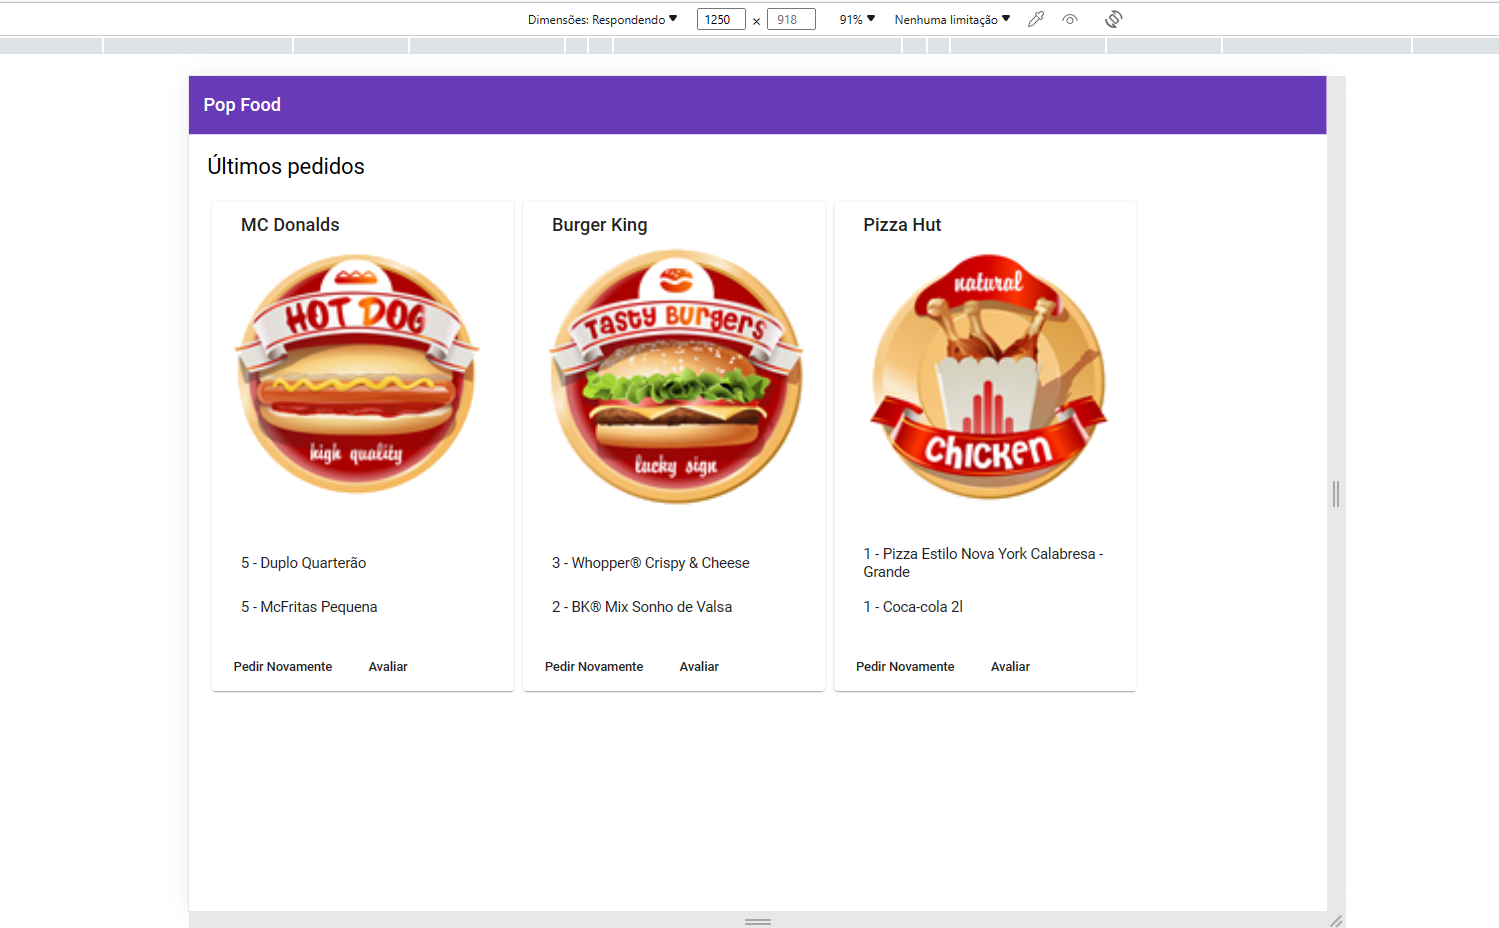
\includegraphics[width=1\textwidth]{front_end_navegador_material.png}
    \caption{Utilização do Angular Material - Visualização Navegador}
    \label{fig:Angular Material}
 \end{figure}

 \begin{figure}[ht]
    \centering
    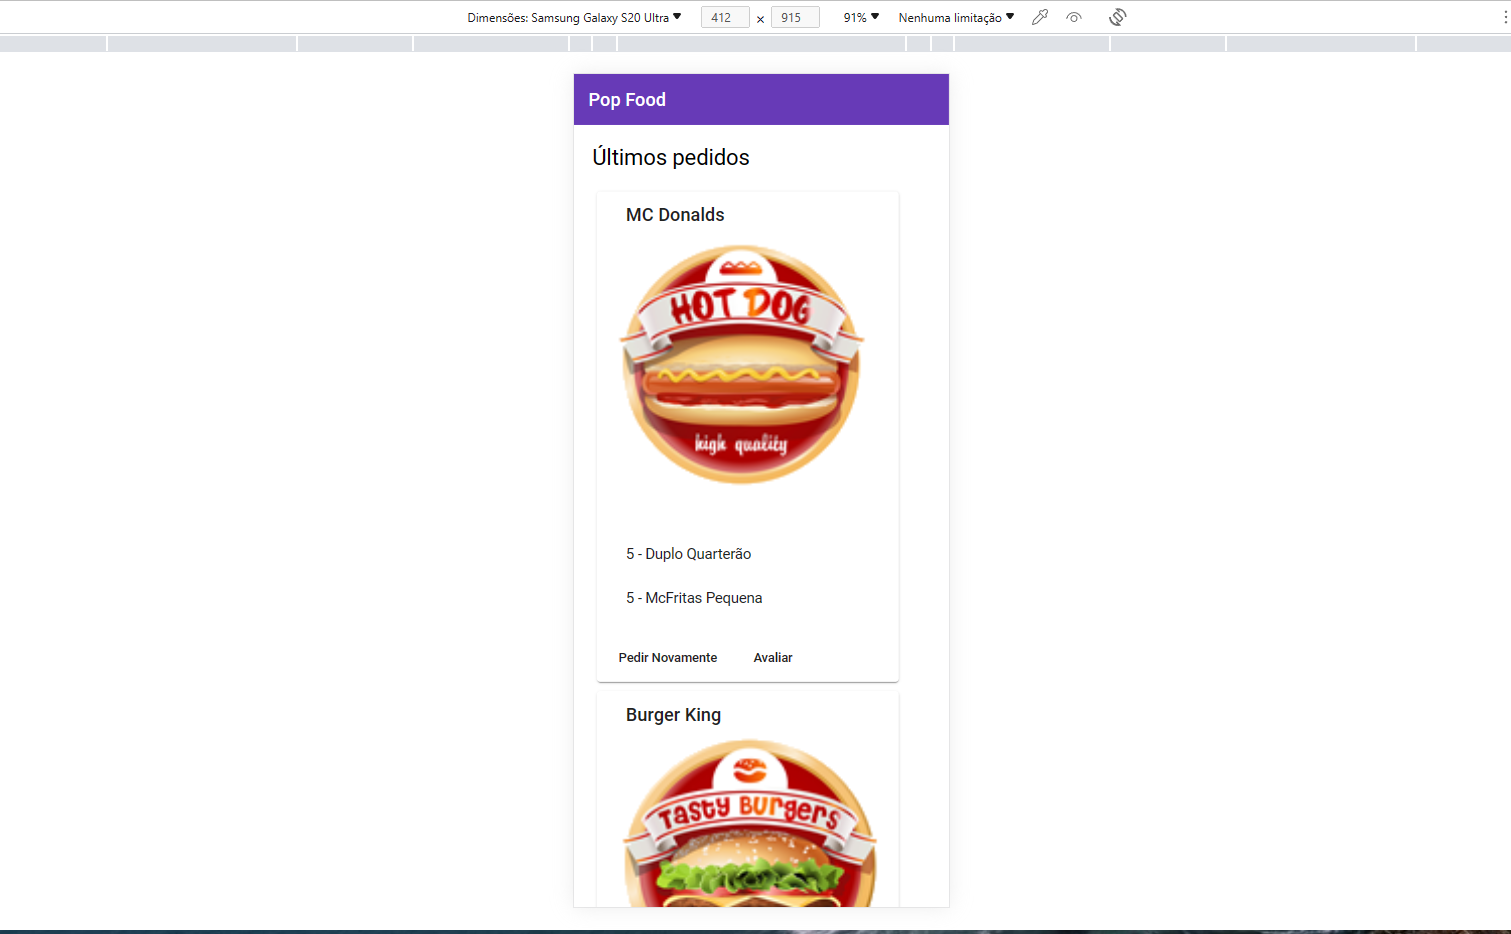
\includegraphics[width=1\textwidth]{front_end_celular_material.png}
    \caption{Utilização do Angular Material - Visualização Celular}
    \label{fig:Angular Material Celular}
 \end{figure}



\pgfmathtruncatemacro\avcen{\avcen + 1}
\subsection{Cenário \avcen} 
\noindent
\begin{tabular}{|>{\raggedright\arraybackslash}p{3cm}|>{\raggedright\arraybackslash}p{10cm}|}
    \hline
    \cellcolor[gray]{0.8}Atributo de Qualidade & Segurança \\
    \hline
    \cellcolor[gray]{0.8}Requisito de Qualidade &  O sistema deverá criptografar dados sensíveis do software, como a senha de acesso do usuário.\\
    \hline
    \multicolumn{2}{|l|}{\cellcolor[gray]{0.8}Preocupação:} \\
    \hline
    \multicolumn{2}{|p{13cm}|}{Proteger informações sensíveis por meio de criptografia para evitar acesso não autorizado aos dados.} \\
    \hline
    \multicolumn{2}{|l|}{\cellcolor[gray]{0.8}Cenário(s):} \\
    \hline
    \multicolumn{2}{|p{13cm}|}{Cenário \avcen} \\
    \hline 
    \multicolumn{2}{|l|}{\cellcolor[gray]{0.8}Ambiente:} \\
    \hline        
    \multicolumn{2}{|p{13cm}|}{Operação normal} \\
    \hline     
    \multicolumn{2}{|l|}{\cellcolor[gray]{0.8}Estímulo:} \\
    \hline  
    \multicolumn{2}{|p{13cm}|}{Tentativa não autorizada de acesso a senha do usuário} \\    
    \hline     
    \multicolumn{2}{|l|}{\cellcolor[gray]{0.8}Mecanismo} \\
    \hline  
    \multicolumn{2}{|p{13cm}|}{Utilização de algoritmos de criptografia para proteger a senha do usuário.} \\
    \hline 
    \multicolumn{2}{|l|}{\cellcolor[gray]{0.8}Medida de Resposta} \\
    \hline            
    \multicolumn{2}{|p{13cm}|}{Dificultar descobrir a senha do usuário.} \\
    \hline 
    \multicolumn{2}{|l|}{\cellcolor[gray]{0.8}Considreação sobre a arquitetura:} \\
    \hline  
    \cellcolor[gray]{0.8}Riscos & Não basta somente criptografar a senha, pois poderão pegar a criptografia e tentar comparar com senhas comuns e então encontrar a senha do usuário, portanto, torna-se necessário acrescentar alguma informação a senha, como um salt(técnica que consiste em adicionar alguma informação secreta a senha, e quando o usuário digitar a senha o sistema acrescenta a informação antes da comparação) que combinado a senha gere a criptografia. \\
    \hline           
    \cellcolor[gray]{0.8}Pontos de Sensibilidade & NA \\
    \hline           
    \cellcolor[gray]{0.8}Tradeoff & NA \\
    \hline         
\end{tabular}

\subsubsection{Evidência do Cenário \avcen} 

No quesito de segurança optou por criptografar os dados sensivéis, a principio foi identificado a senha como uma informação sensível, sendo necessário 
avaliar as demais informações para definir o que deve ser criptografado.

\begin{figure}[ht]
    \centering
    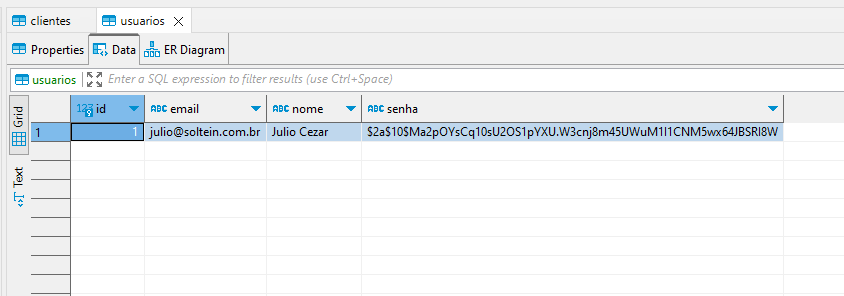
\includegraphics[width=1\textwidth]{senha_criptografada.png}
    \caption{Segurança criptografia senha}
    \label{fig:Segurança criptografia senha}
 \end{figure}

\pgfmathtruncatemacro\avcen{\avcen + 1}
\subsection{Cenário \avcen} 
\noindent
\begin{tabular}{|>{\raggedright\arraybackslash}p{3cm}|>{\raggedright\arraybackslash}p{10cm}|}
    \hline
    \cellcolor[gray]{0.8}Atributo de Qualidade & Segurança \\
    \hline
    \cellcolor[gray]{0.8}Requisito de Qualidade &  Ao tentar acessar um recurso privado sem estar logado, o sistema deverá exibir uma mensagem de não autorizado.\\
    \hline
    \multicolumn{2}{|l|}{\cellcolor[gray]{0.8}Preocupação:} \\
    \hline
    \multicolumn{2}{|p{13cm}|}{Garantir que somente usuários autorizados tenham acesso aos recursos privados.} \\
    \hline
    \multicolumn{2}{|l|}{\cellcolor[gray]{0.8}Cenário(s):} \\
    \hline
    \multicolumn{2}{|p{13cm}|}{Cenário \avcen} \\
    \hline 
    \multicolumn{2}{|l|}{\cellcolor[gray]{0.8}Ambiente:} \\
    \hline        
    \multicolumn{2}{|p{13cm}|}{Operação normal} \\
    \hline     
    \multicolumn{2}{|l|}{\cellcolor[gray]{0.8}Estímulo:} \\
    \hline  
    \multicolumn{2}{|p{13cm}|}{Tentativa de acesso a recurso privado sem estar logado} \\    
    \hline     
    \multicolumn{2}{|l|}{\cellcolor[gray]{0.8}Mecanismo} \\
    \hline  
    \multicolumn{2}{|p{13cm}|}{Implementação de um controle de autenticação e autorização que verifica se o usuário está logado e possui as permissões necessárias para acessar o recurso.} \\
    \hline 
    \multicolumn{2}{|l|}{\cellcolor[gray]{0.8}Medida de Resposta} \\
    \hline            
    \multicolumn{2}{|p{13cm}|}{Não autorizar acesso a recursos privados do software.} \\
    \hline 
    \multicolumn{2}{|l|}{\cellcolor[gray]{0.8}Consideração sobre a arquitetura:} \\
    \hline  
    \cellcolor[gray]{0.8}Riscos &  Implementação de um controle de autenticação e autorização que verifica se o usuário está logado e possui as permissões necessárias para acessar o recurso. \\
    \hline           
    \cellcolor[gray]{0.8}Pontos de Sensibilidade & NA \\
    \hline           
    \cellcolor[gray]{0.8}Tradeoff & NA \\
    \hline         
\end{tabular}

\subsubsection{Evidência do Cenário \avcen} 

Neste quesito foi desenvolvido um módulo de autenticação baseado em JWT(JSON Web Token), pois ele é utilizado amplamente 
em autenticação de sistemas, o back end ao receber os dados de acesso gera um token temporário que permite ao usuário acessar 
áreas privadas do sistema.

\begin{figure}[ht]
    \centering
    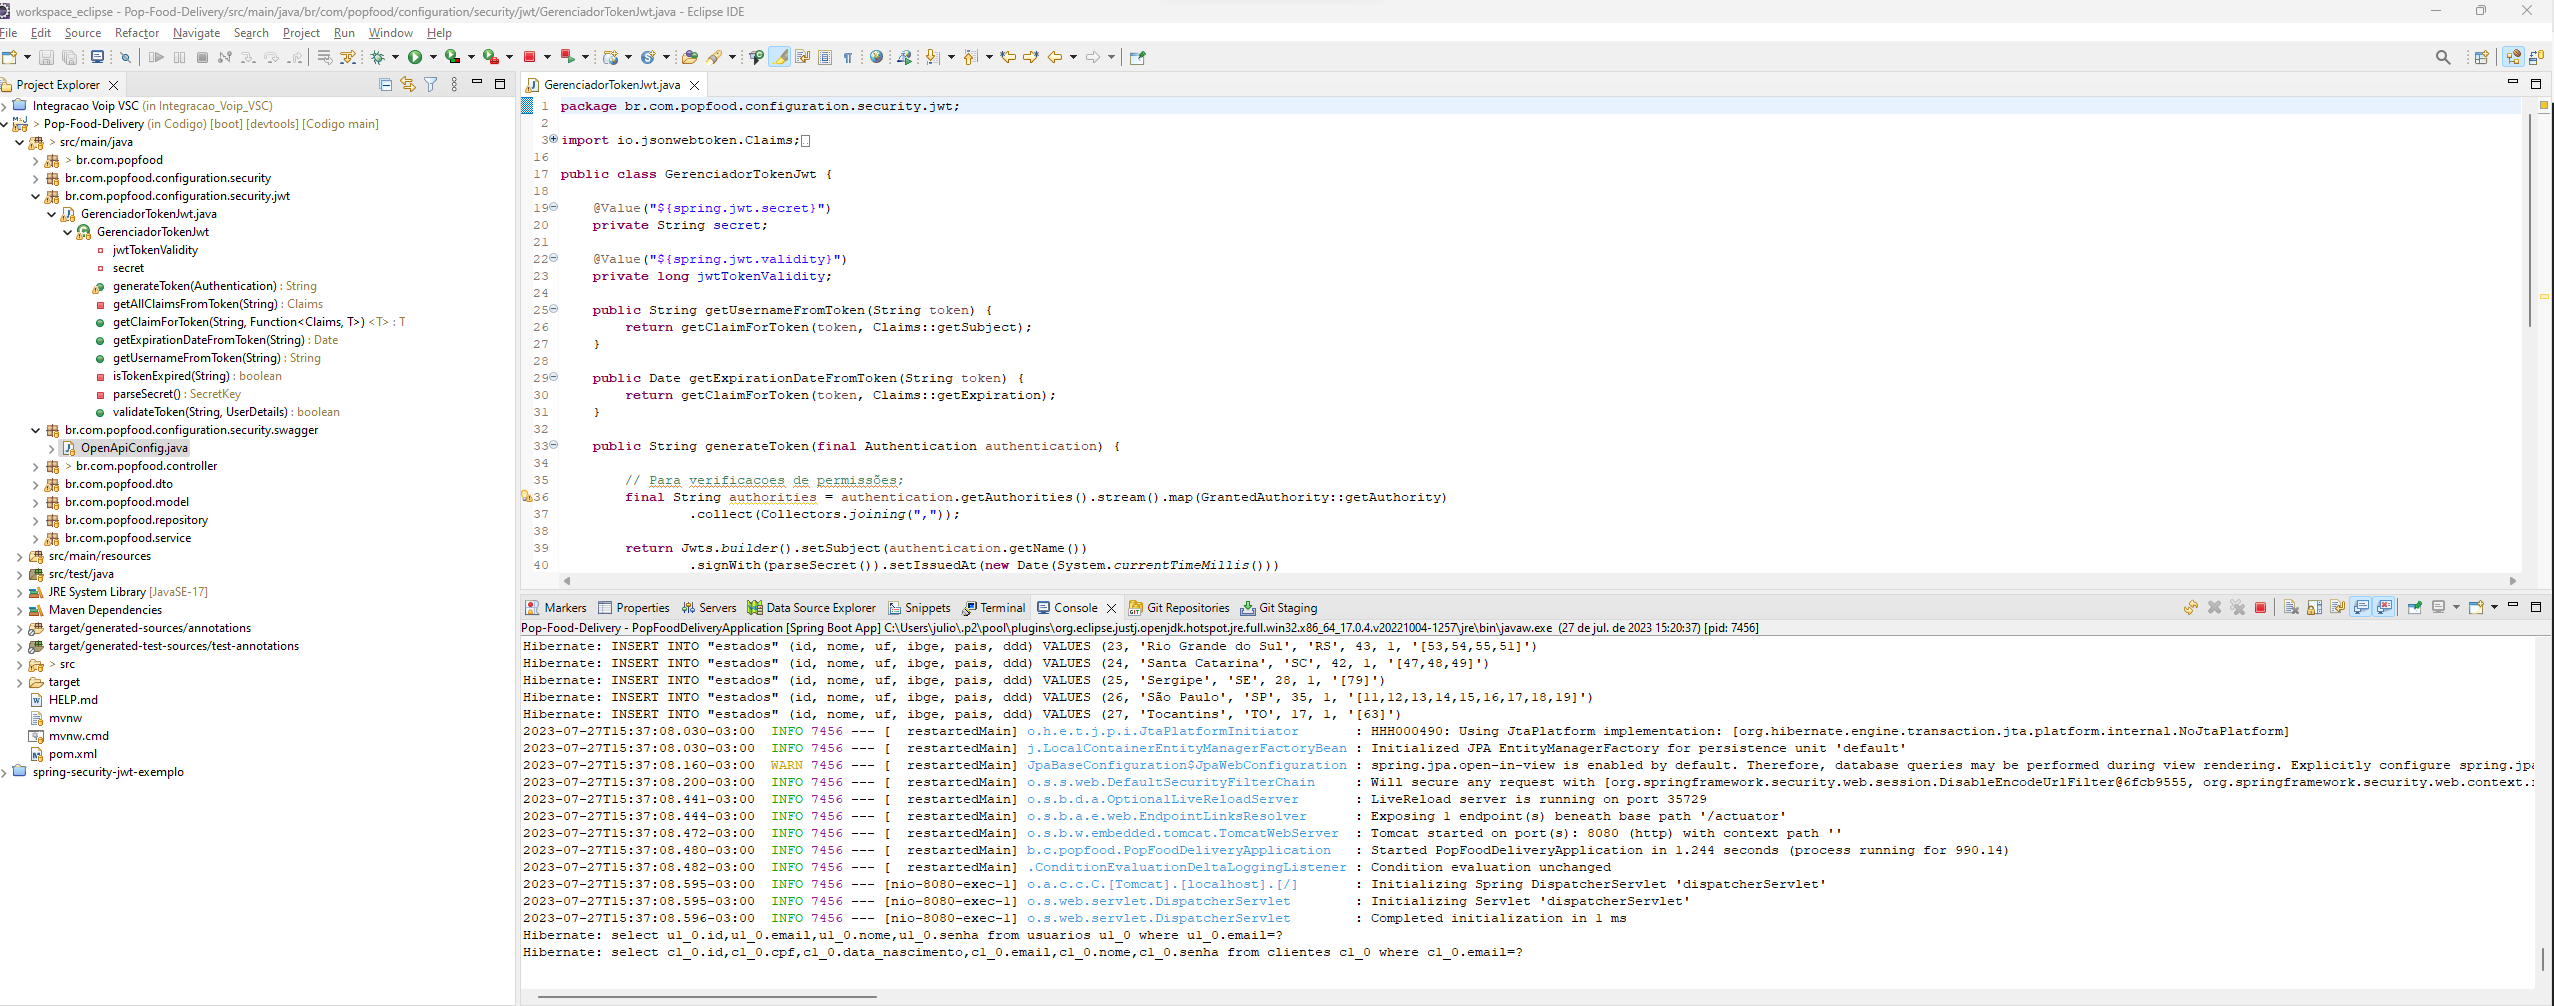
\includegraphics[width=1\textwidth]{codigo_fonte_jwt.png}
    \caption{Parte do código responsável pelo JWT.}
    \label{fig:Parte do código responsável pelo JWT.}
 \end{figure}

\begin{figure}[ht]
    \centering
    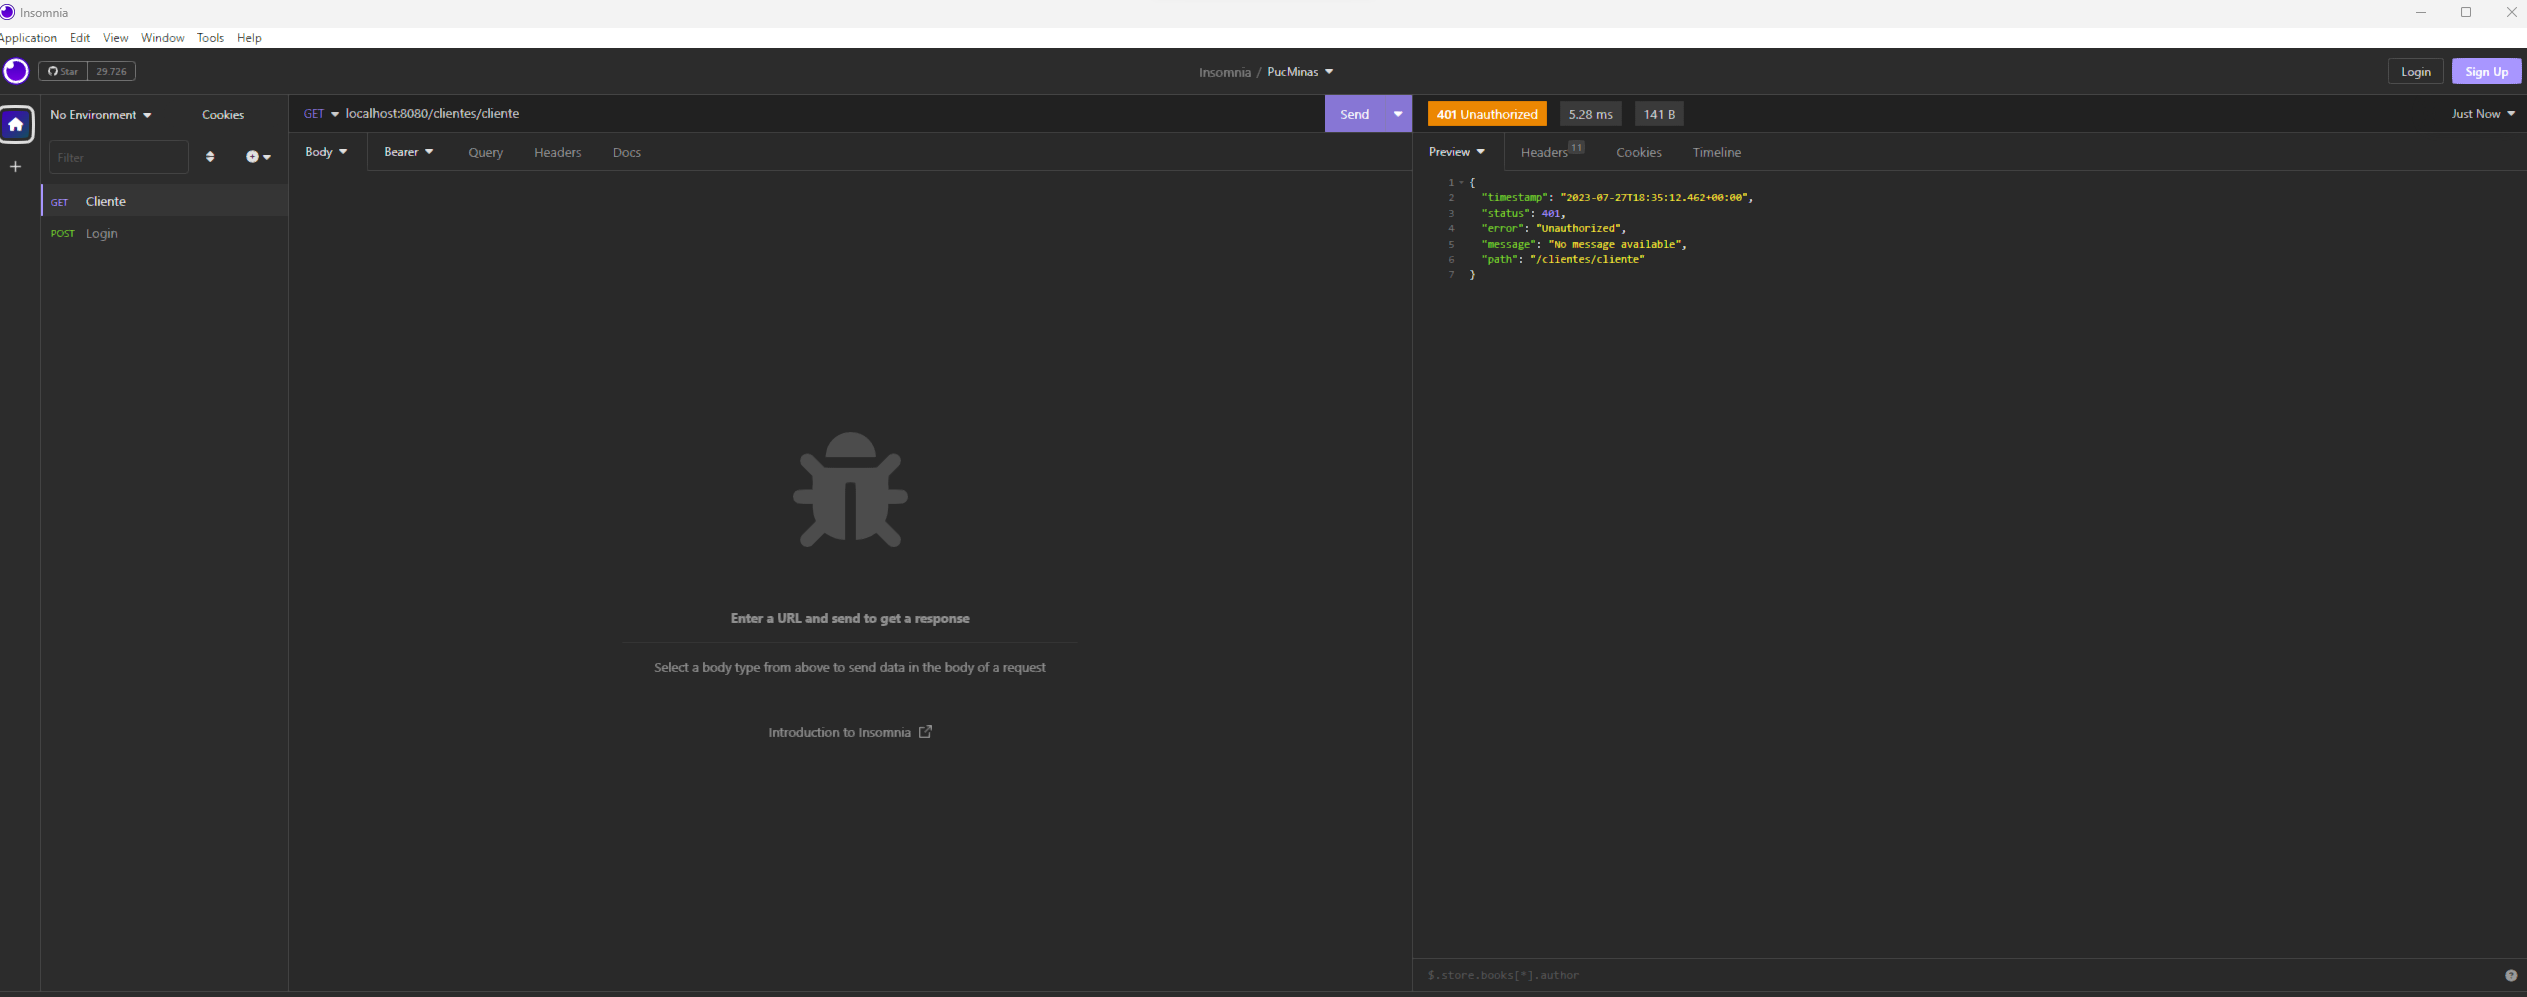
\includegraphics[width=1\textwidth]{acesso_sem_token.png}
    \caption{Tentativa de acesso sem estar logado.}
    \label{fig:Tentativa de acesso sem estar logado.}
 \end{figure}

 \begin{figure}[ht]
    \centering
    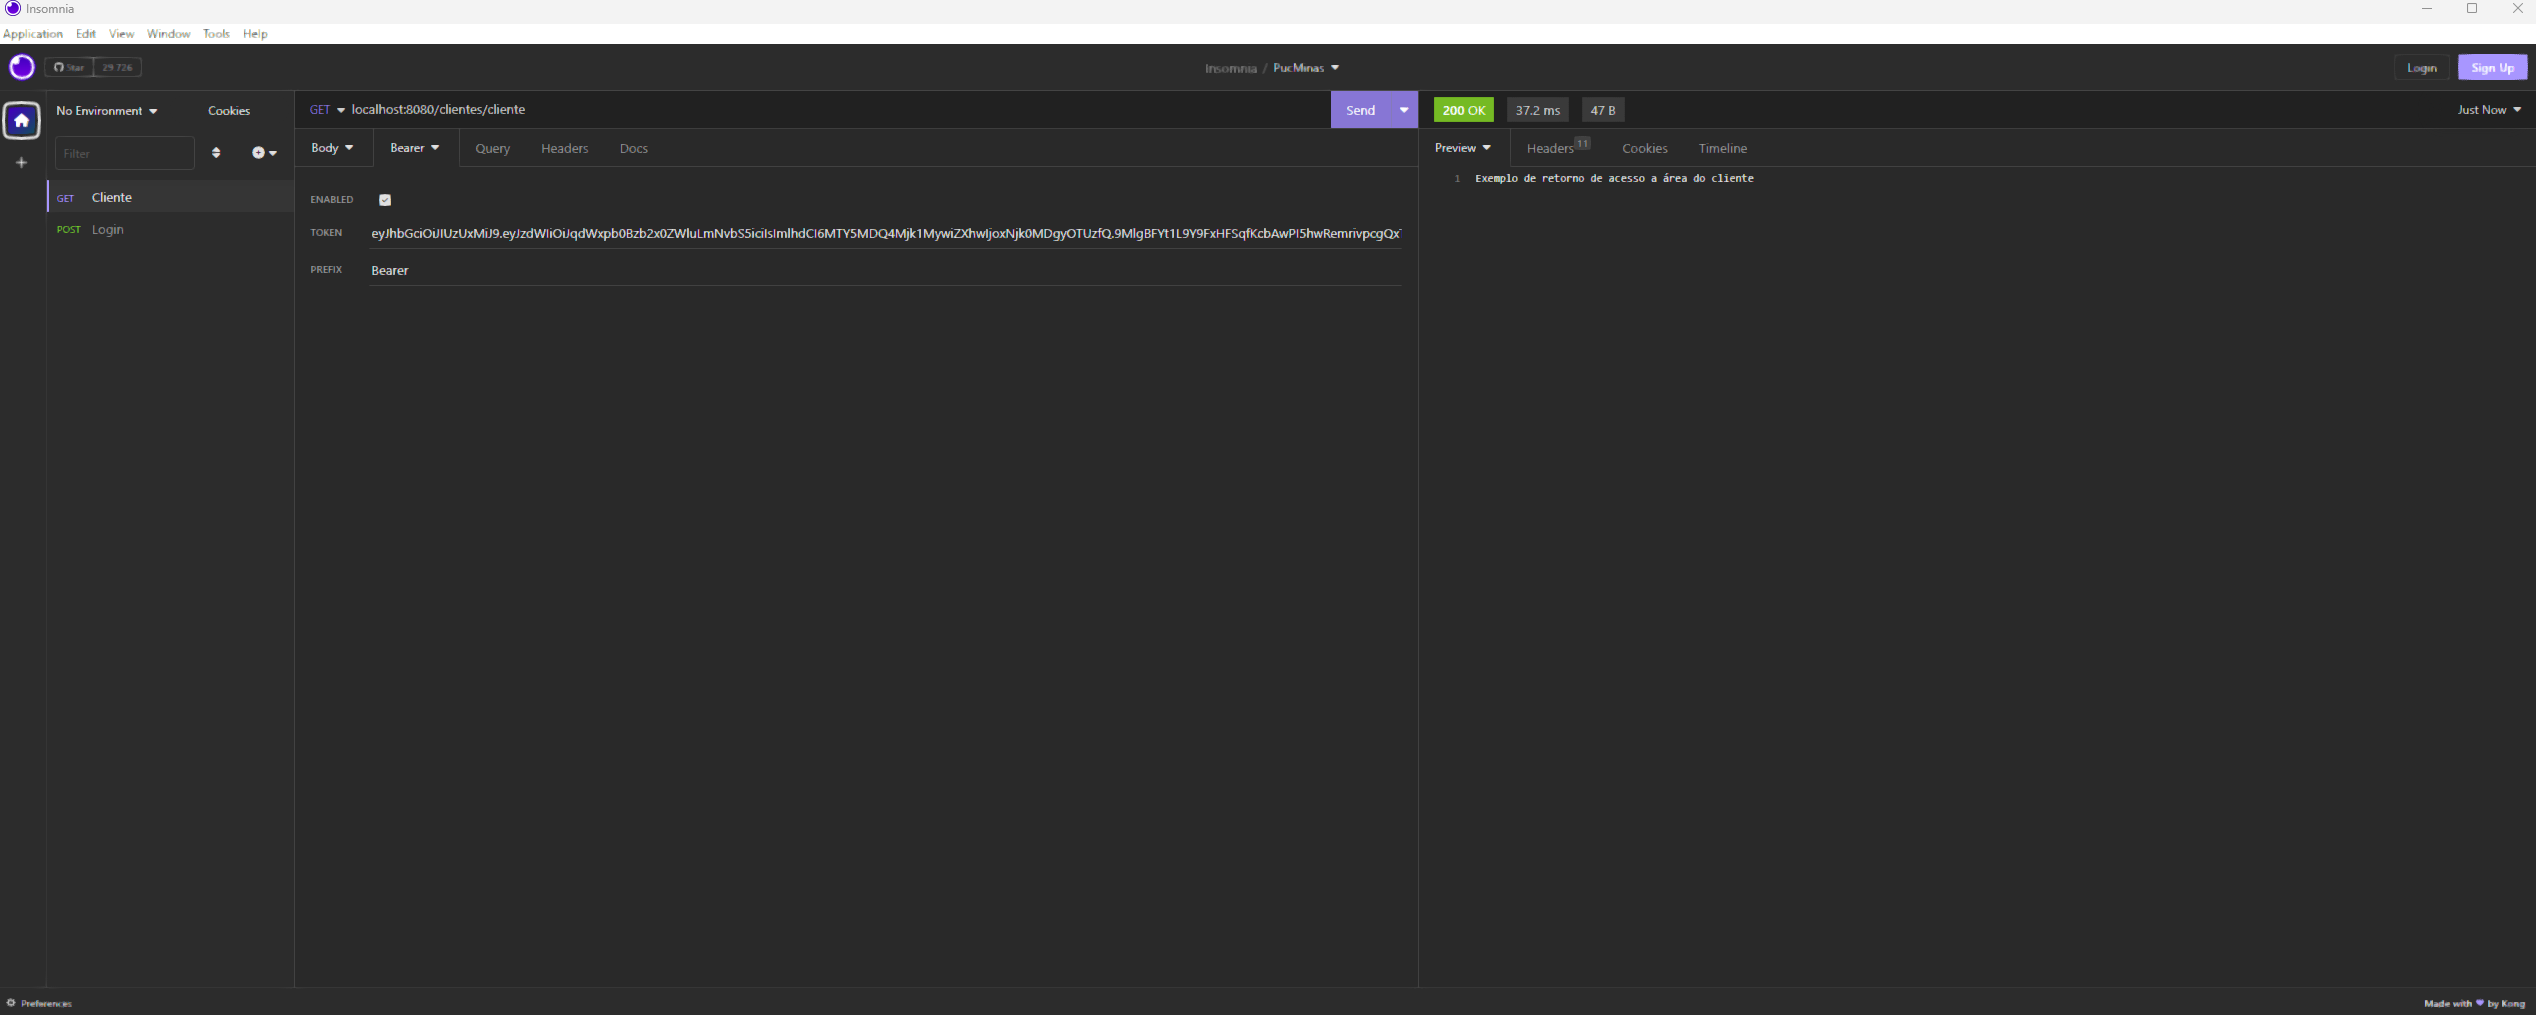
\includegraphics[width=1\textwidth]{acesso_com_token.png}
    \caption{Tentativa de acesso logado ao sistema.}
    \label{fig:Tentativa de acesso logao ao sistema.}
 \end{figure}



 \pgfmathtruncatemacro\avcen{\avcen + 1}
 \subsection{Cenário \avcen} 
 \noindent
 \begin{tabular}{|>{\raggedright\arraybackslash}p{3cm}|>{\raggedright\arraybackslash}p{10cm}|}
     \hline
     \cellcolor[gray]{0.8}Atributo de Qualidade & Interoperabilidade \\
     \hline
     \cellcolor[gray]{0.8}Requisito de Qualidade &  O sistema deve considerar a capacidade de se comunicar com outros sistemas de software em outras tecnologias, adotando padrões de comunicação amplamente aceitos, como RESTful, utilizando formatos de dados amplamente utilizados como JSON.\\
     \hline
     \multicolumn{2}{|l|}{\cellcolor[gray]{0.8}Preocupação:} \\
     \hline
     \multicolumn{2}{|p{13cm}|}{Garantir que o sistema possa integrar-se com outros sistemas de software, utilizando padrões amplamente adotados no mercado.} \\
     \hline
     \multicolumn{2}{|l|}{\cellcolor[gray]{0.8}Cenário(s):} \\
     \hline
     \multicolumn{2}{|p{13cm}|}{Cenário \avcen} \\
     \hline 
     \multicolumn{2}{|l|}{\cellcolor[gray]{0.8}Ambiente:} \\
     \hline        
     \multicolumn{2}{|p{13cm}|}{Operação normal} \\
     \hline     
     \multicolumn{2}{|l|}{\cellcolor[gray]{0.8}Estímulo:} \\
     \hline  
     \multicolumn{2}{|p{13cm}|}{Necessidade do cliente efetuar um pagamento online do pedido.} \\    
     \hline     
     \multicolumn{2}{|l|}{\cellcolor[gray]{0.8}Mecanismo} \\
     \hline  
     \multicolumn{2}{|p{13cm}|}{Utilização de protocolos de comunicação amplamente aceitos, como RESTful, para integrar com o meio de pagamento externo.} \\
     \hline 
     \multicolumn{2}{|l|}{\cellcolor[gray]{0.8}Medida de Resposta} \\
     \hline            
     \multicolumn{2}{|p{13cm}|}{Sucesso na comunicação e integração com o meio de pagamento externo, evidenciado pela realização bem-sucedida de transações e processamentos de pagamento.} \\
     \hline 
     \multicolumn{2}{|l|}{\cellcolor[gray]{0.8}Consideração sobre a arquitetura:} \\
     \hline  
     \cellcolor[gray]{0.8}Riscos & Os sistemas podem estar vulneráveis a ameaças de segurança, levando ao comprometimento de dados e roubos de informações sensíveis, principalmente por se tratar
     de dados de pagamento. Portanto é necessário verificar as diversas possibilidades, como a tela em que o usuário digita as informações de cartão já ser uma tela da operadora, dessa forma não teremos a responsabilidade sobre as informações. \\
     \hline           
     \cellcolor[gray]{0.8}Pontos de Sensibilidade & Um dos principais pontos de sensibilidade é o armazenamento das informações de cartões, deve-se decidir se essas informações ficarão armazenadas ou se encontrará uma operadora em que os dados sejam digitados em seu sistema.
     Caso opte por armazenar, é necessário uma evolução maior da arquitetura pois ai iremos tratar de implementações como certificação PCI o que aumenta a complexidade do sistema e infra-estrutura. \\
     \hline           
     \cellcolor[gray]{0.8}Tradeoff & É importante equilibrar a segurança com os desejos de funcionalidades do sistema, é de grande desejo ter a opção de pagamento online, mas devemos ter uma visão 
     sobre a segurança desta funcionalidade e o riscos e prejuízos em casos de falha. Portanto é necessário encontrar um meio termo como informado anteriormente, uma plataforma que já tenha esse nível de segurança garantido e processamos somente 
     enviar dados não sensíveis e esta plataforma cuidar das informações mais sensíveis como dados de cartão. \\
     \hline         
 \end{tabular}
 
 \subsubsection{Evidência do Cenário \avcen} 

 Foi desenvolvido um POC para simular a integração com a CIELO, utilizamos da documentação deles e desenvolvemos um exemplo fictício com o objetivo de testar a 
 tecnologia utilizada, no caso RestTemplet do Spring. 

 Neste POC criamos uma chamada ao end point da CIELO passando as informações via JSON e obtemos o retorno de sucesso da geração do pedido de compra nos sistemas deles.


 \begin{figure}[ht]
    \centering
    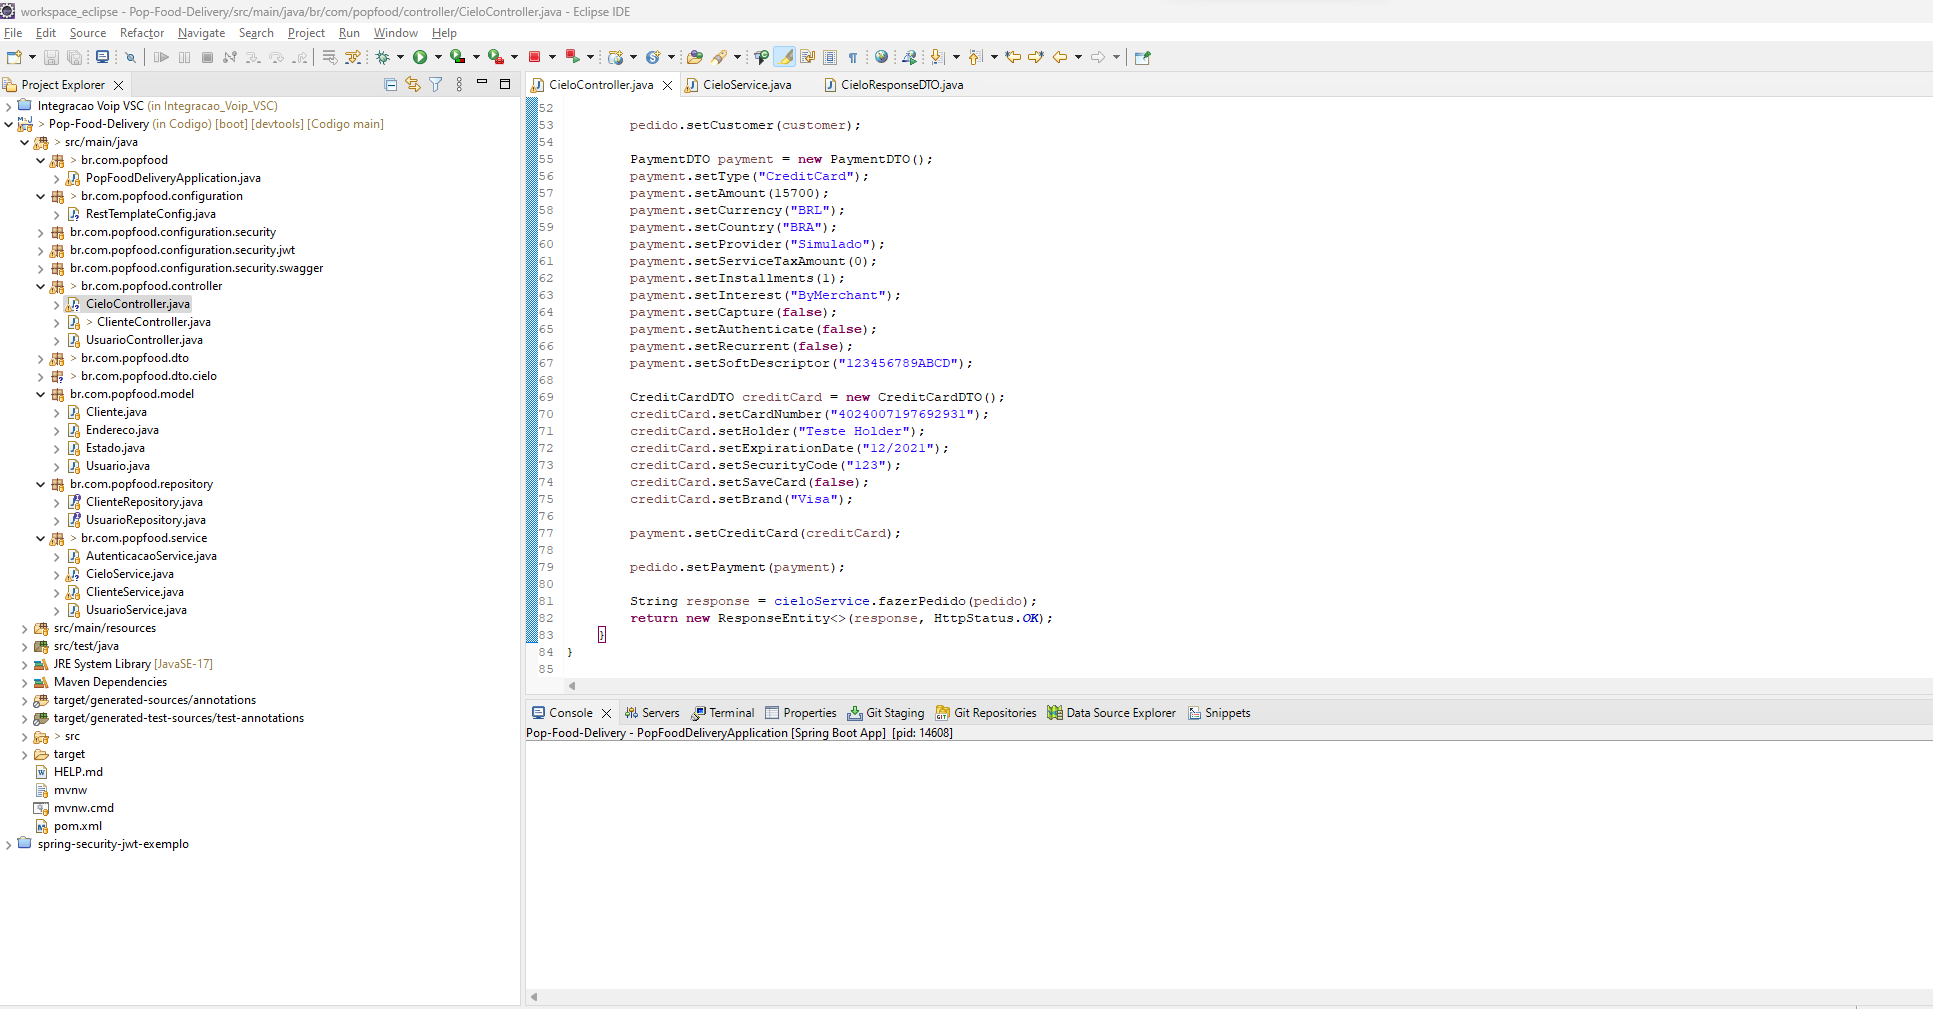
\includegraphics[width=1\textwidth]{interoperabilidade_cielo_controller.png}
    \caption{Código fonte controller POC - CIELO.}
    \label{fig:Código fonte controller POC - CIELO.}
 \end{figure}

 \begin{figure}[ht]
    \centering
    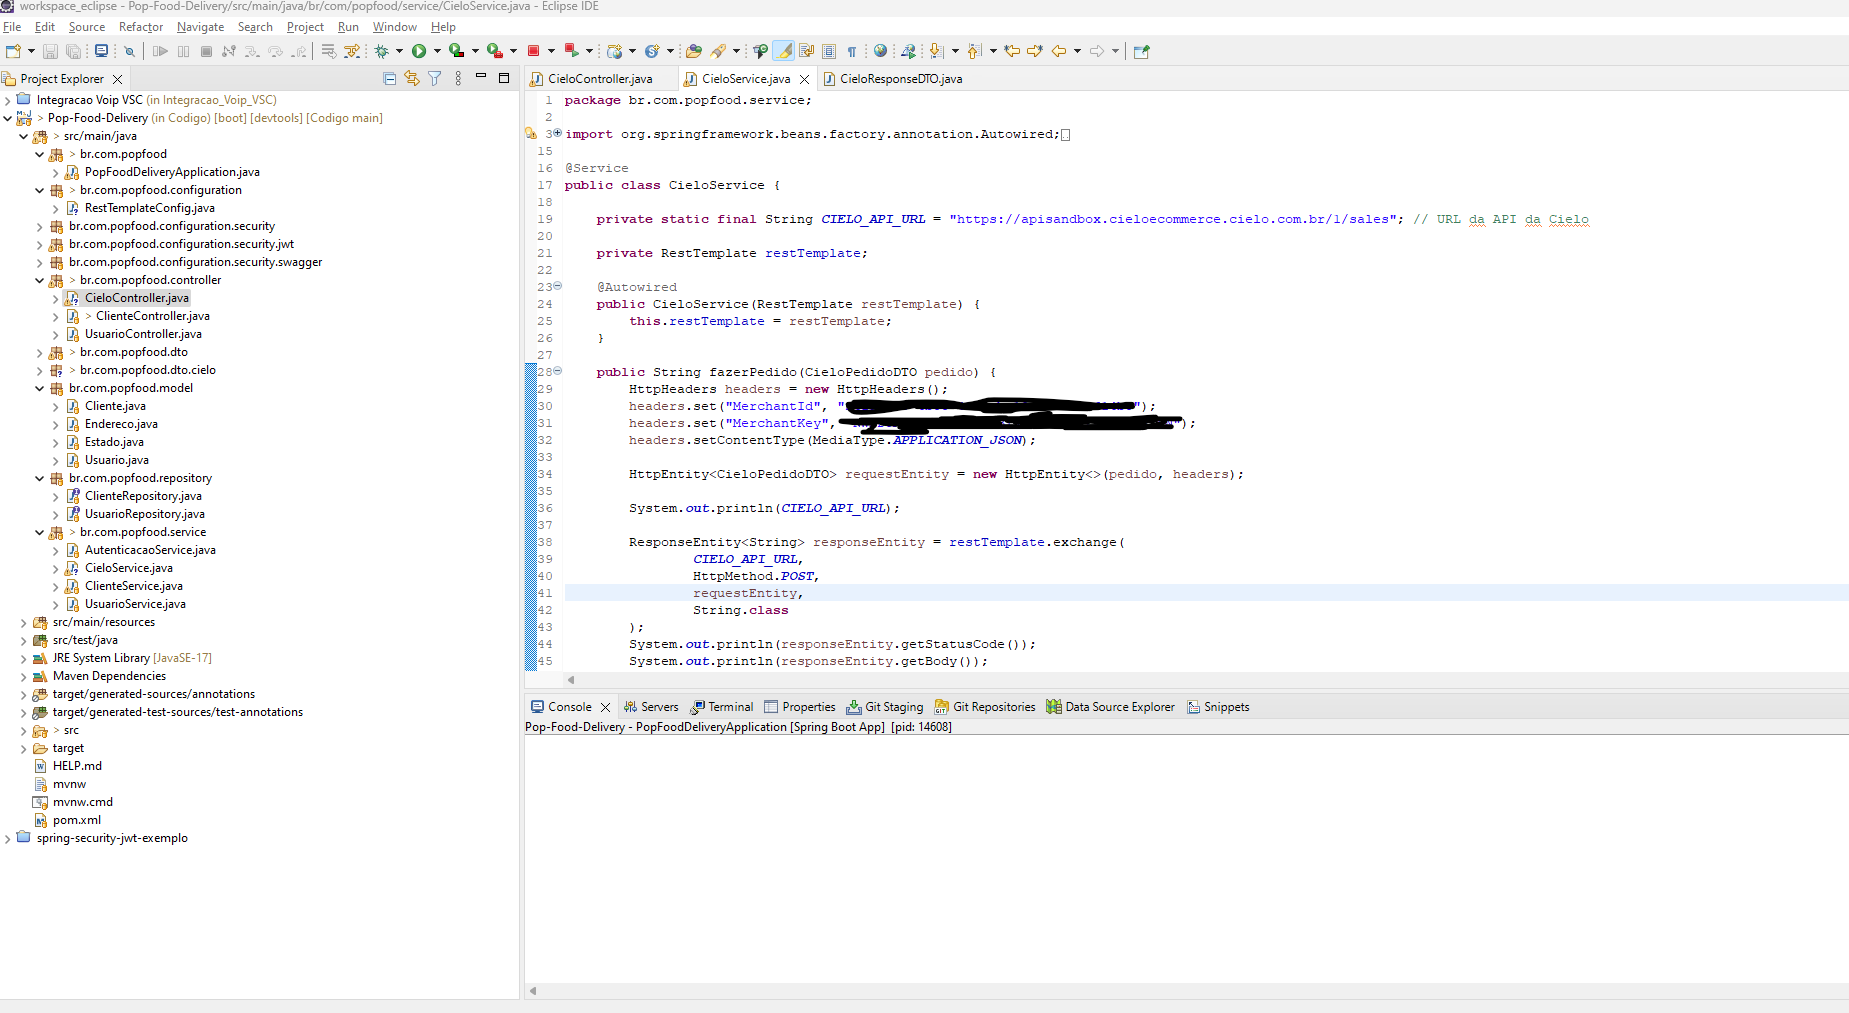
\includegraphics[width=1\textwidth]{interoperabilidade_cielo_service.png}
    \caption{Código fonte service POC - CIELO.}
    \label{fig:Código fonte service POC - CIELO.}
 \end{figure}

 \begin{figure}[ht]
    \centering
    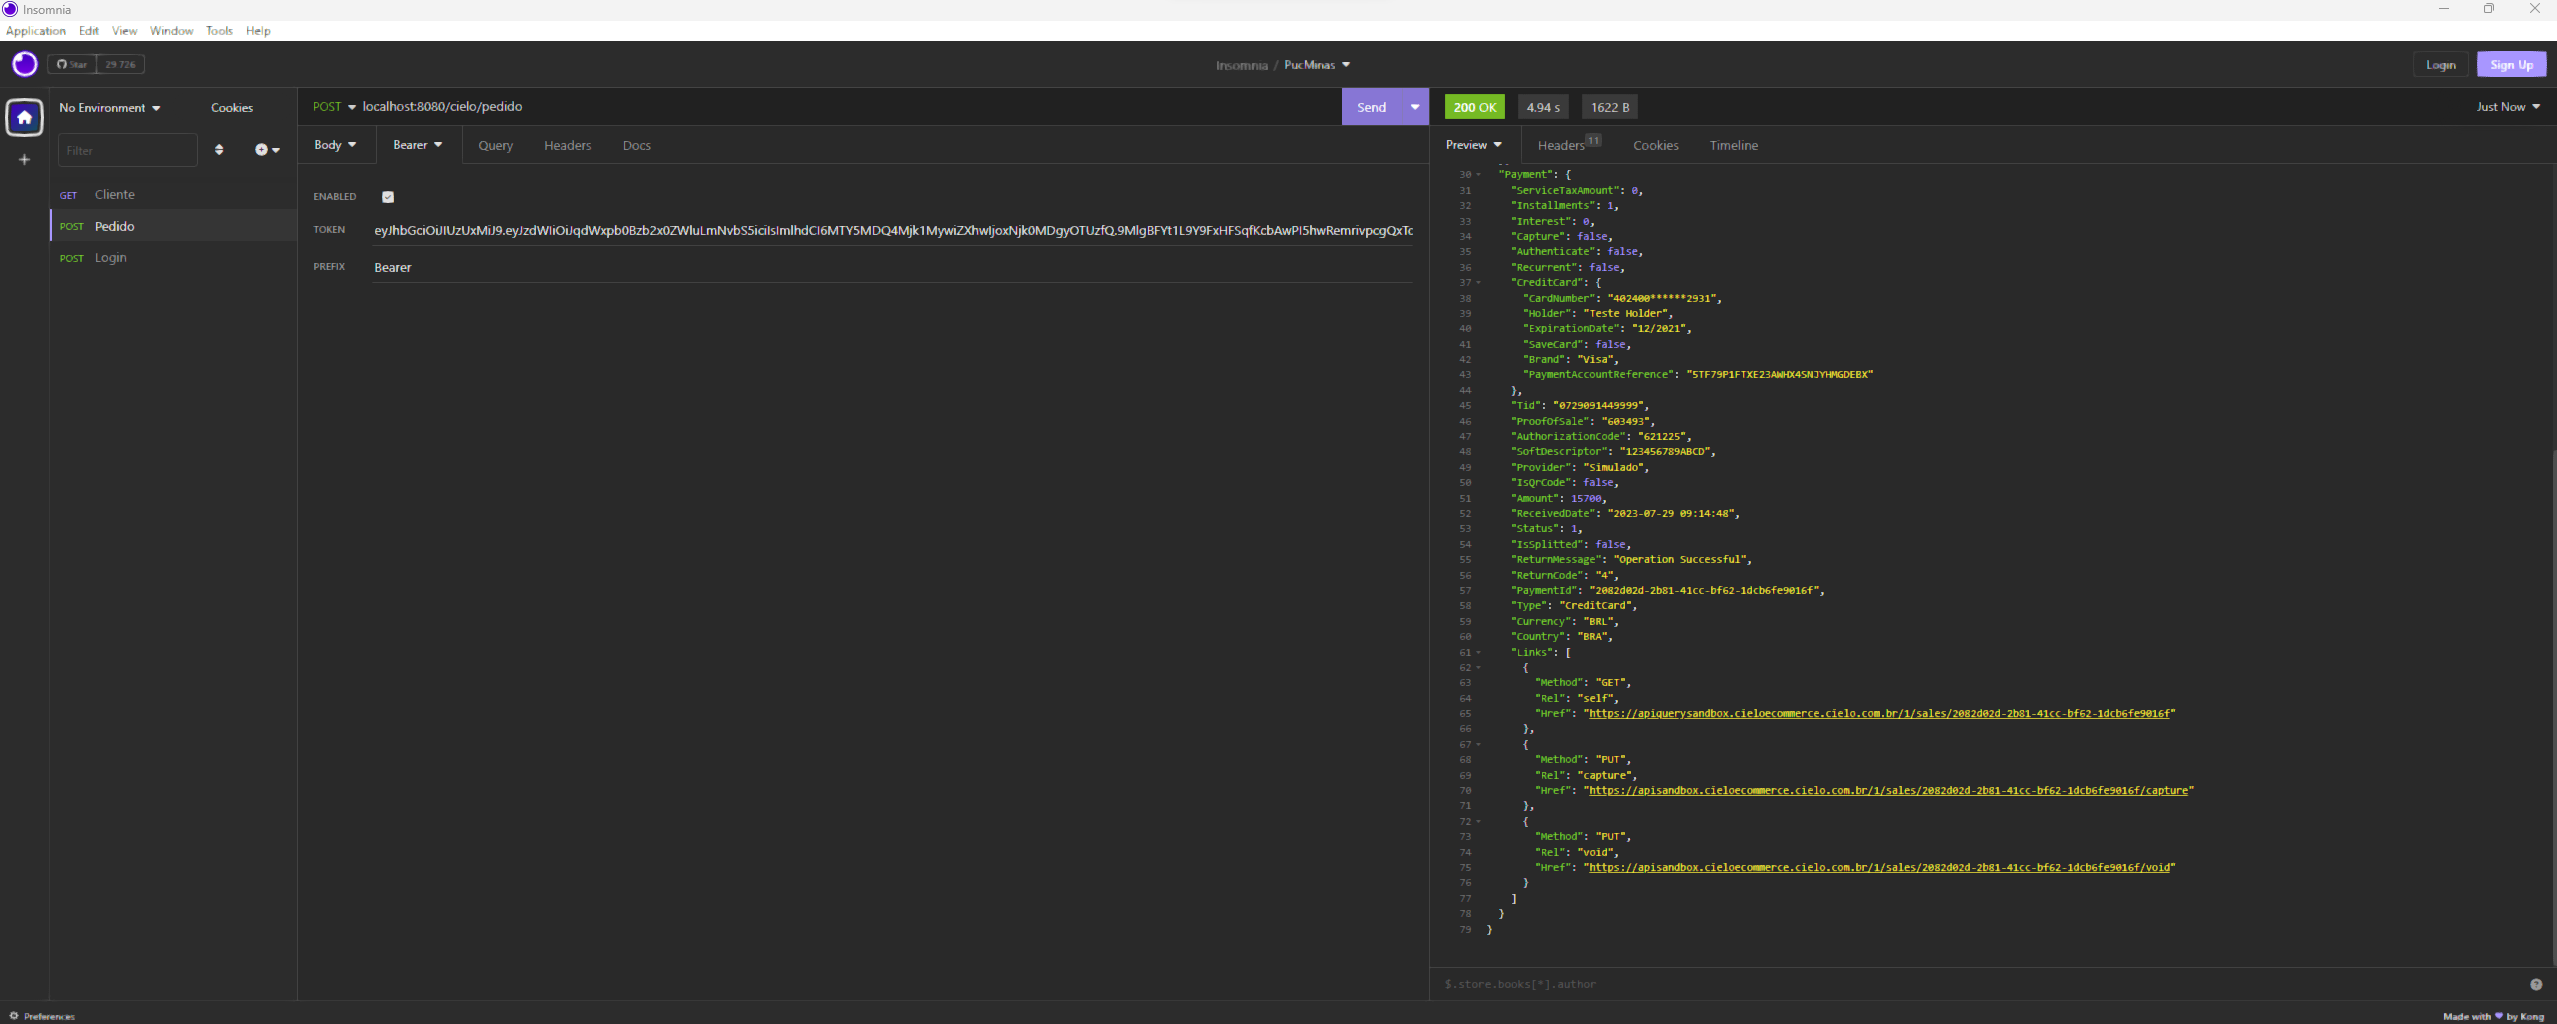
\includegraphics[width=1\textwidth]{interoperabilidade_retorno_insominia.png}
    \caption{Teste de execução com INSOMINIA POC - CIELO.}
    \label{fig:Teste de execução com INSOMINIA POC - CIELO.}
 \end{figure}



 \pgfmathtruncatemacro\avcen{\avcen + 1}
 \subsection{Cenário \avcen} 
 \noindent
 \begin{tabular}{|>{\raggedright\arraybackslash}p{3cm}|>{\raggedright\arraybackslash}p{10cm}|}
     \hline
     \cellcolor[gray]{0.8}Atributo de Qualidade & Desempenho \\
     \hline
     \cellcolor[gray]{0.8}Requisito de Qualidade &   O sistema deve ser capaz de exibir sua tela inicial após a inserção dos dados de acesso em menos de 5 segundos.\\
     \hline
     \multicolumn{2}{|l|}{\cellcolor[gray]{0.8}Preocupação:} \\
     \hline
     \multicolumn{2}{|p{13cm}|}{Garantir que o sistema ofereça uma experiência fluida para o usuário ao efetuar o login, proporcionando tempo de resposta rápido e eficiente.} \\
     \hline
     \multicolumn{2}{|l|}{\cellcolor[gray]{0.8}Cenário(s):} \\
     \hline
     \multicolumn{2}{|p{13cm}|}{Cenário \avcen} \\
     \hline 
     \multicolumn{2}{|l|}{\cellcolor[gray]{0.8}Ambiente:} \\
     \hline        
     \multicolumn{2}{|p{13cm}|}{Operação normal} \\
     \hline     
     \multicolumn{2}{|l|}{\cellcolor[gray]{0.8}Estímulo:} \\
     \hline  
     \multicolumn{2}{|p{13cm}|}{Efetuar login no sistema.} \\    
     \hline     
     \multicolumn{2}{|l|}{\cellcolor[gray]{0.8}Mecanismo} \\
     \hline  
     \multicolumn{2}{|p{13cm}|}{Implementação de estratégia de autenticação otimizada baseada em usuário e senha. Utilização de JTW para geração de token a ser validado nas rotas privadas da aplicação.} \\
     \hline 
     \multicolumn{2}{|l|}{\cellcolor[gray]{0.8}Medida de Resposta} \\
     \hline            
     \multicolumn{2}{|p{13cm}|}{Tempo de resposta na geração do TOKEN de acesso as demais telas do sistema.} \\
     \hline 
     \multicolumn{2}{|l|}{\cellcolor[gray]{0.8}Consideração sobre a arquitetura:} \\
     \hline  
     \cellcolor[gray]{0.8}Riscos & Uma sobrecarga do servidor em caso de grande número de acessos simultâneos poderá acarretar em degradação do desempenho do sistema como um todo. \\
     \hline           
     \cellcolor[gray]{0.8}Pontos de Sensibilidade &  NA\\
     \hline           
     \cellcolor[gray]{0.8}Tradeoff & NA \\
     \hline         
 \end{tabular}
 
 \subsubsection{Evidência do Cenário \avcen} 

 Foi efetuada a simulação de acesso ao sistema utilizando o INSOMINIA, nele foi verificado que o sistema em operação normal 
 o acesso é muito rápido, ficando em 82.4 ms. É claro que no uso diário do sistema deverá ser acompanhado o crescimento do mesmo e a 
 quantidade de usuários simultâneos, e caso necessário a infra-estrutura deverá crescer vertical e horizontalmente para atender a demanda.

 \begin{figure}[ht]
    \centering
    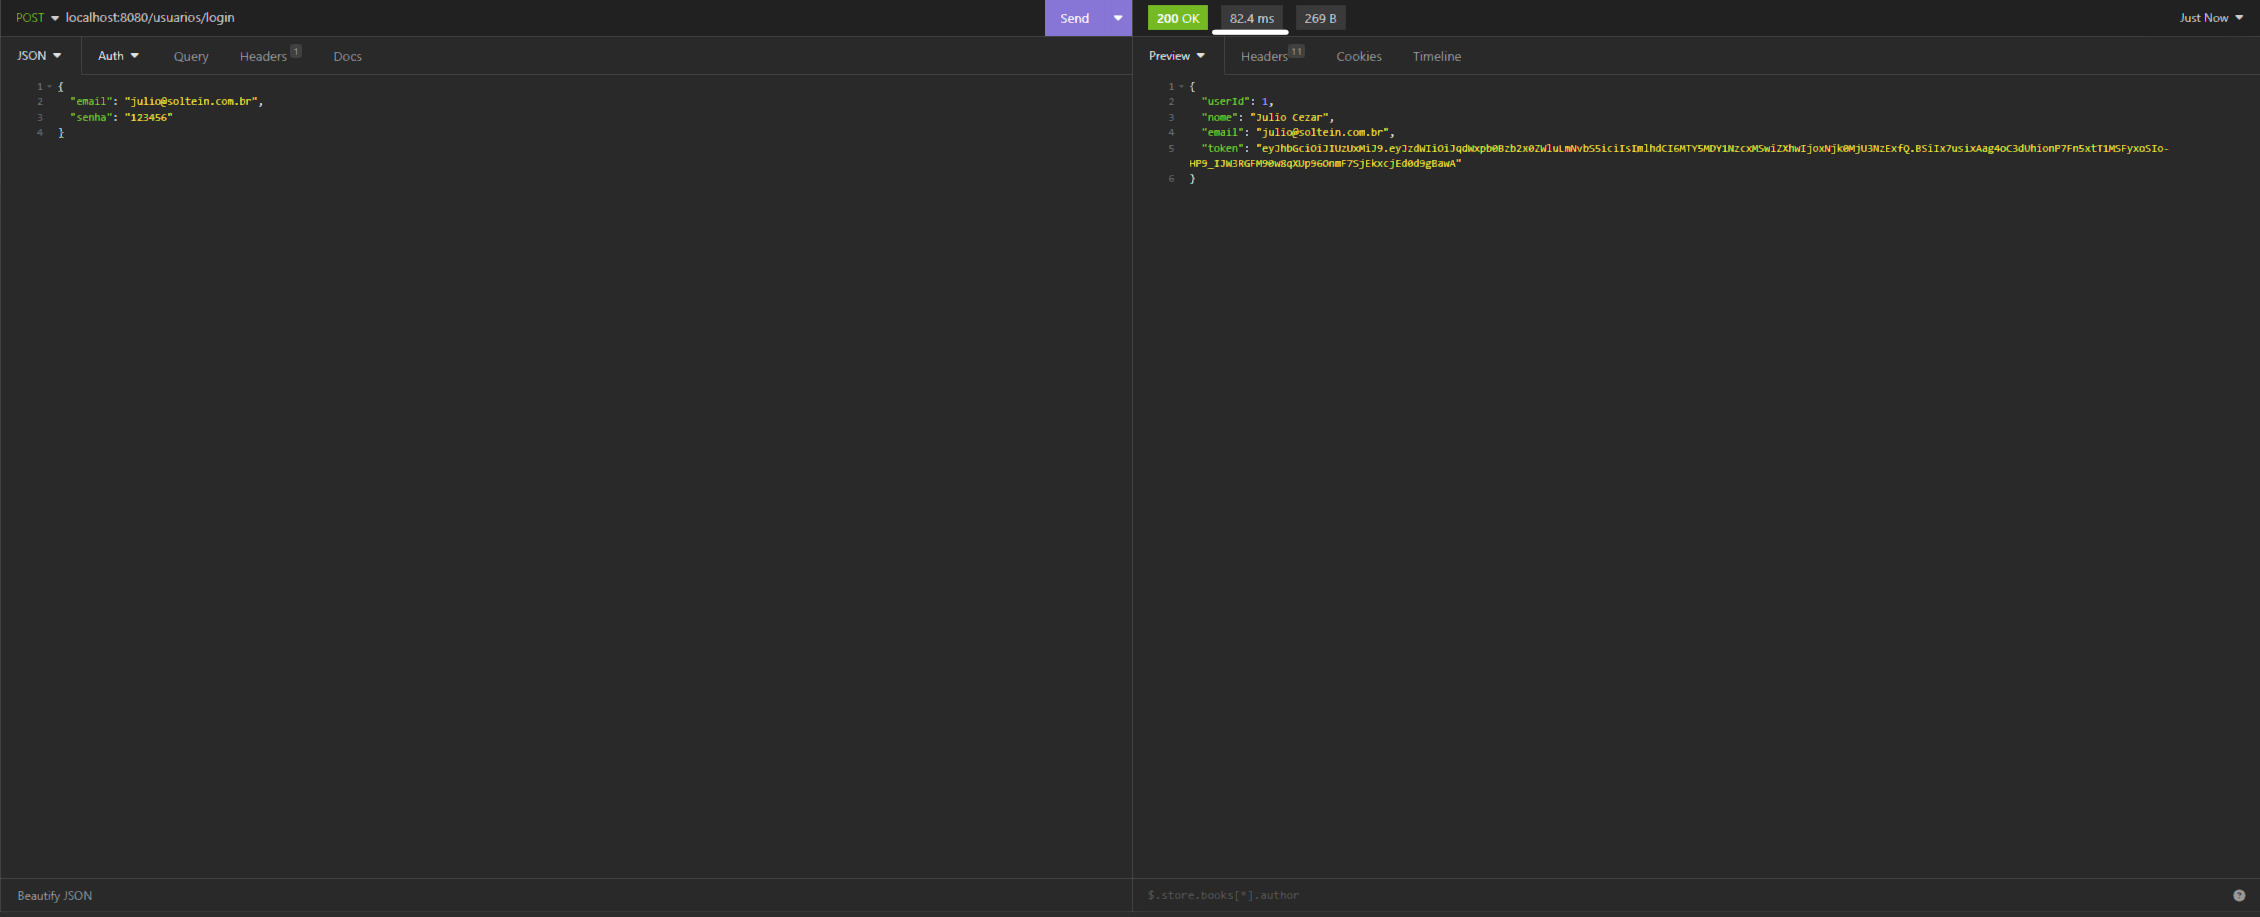
\includegraphics[width=1\textwidth]{desempenho.png}
    \caption{Tempo de resposta para acesso ao sistema. 82.4ms.}
    \label{fig:Tempo de resposta para acesso ao sistema. 82.4ms.}
 \end{figure}

 \chapter{Avaliação crítica dos resultados}

 De acordo com a proposta do projeto, podemos verificar que os requisitos não funcionais foram atendidos e validados com sucesso, mas há margem para melhorias como por exemplo em relação a integração com 
 operadora de pagamento online, deve-se focar na parte de segurança, fazendo um estudo mais aplicado nas opções de mercado antes de se optar por alguma.

 \noindent
 \begin{tabular}{|>{\raggedright\arraybackslash}p{4cm}|>{\raggedright\arraybackslash}p{10cm}|}
    \hline
    \cellcolor[gray]{0.8}Ponto Avaliado & \cellcolor[gray]{0.8}Descrição \\
    Arquitetura MVC & A utilização do padrão MVC permitiu que as responsabilidades do sistema fossem separadas de forma clara, isto irá facilitar a manutenção e evolução do mesmo. No entanto poderão surgir desafios em relação a manter a organização em camadas na medida que a equipe crescer, exigindo uma maior coordenação do desenvolvimento.\\
    \hline
    Usabilidade & Ao utilizar o Material Angular mantemos a padronização dos componentes de interface, e utilizamos recursos já utilizados em diversos aplicativos de software,
    isto permite manter uma facilidade de aprendizado para o usuário além de compatibilidade com diferentes resoluções. Como no desenvolvimento em camadas, a utilização do Material Angular
    requer que a equipe mantenha-se no propósito de utilizar o mesmo, sendo necessário novamente uma boa coordenação de equipe.\\
    \hline
    Segurança & No quesito de segurança garantimos a proteção de dados sensíveis através de criptografia e controle de acesso adequado. Mas ainda é necessário
    se atentar a outros quesitos como na questão de pagamentos online no que se refere a dados de cartão e também ao armazenamento do token de acesso.\\
    \hline
    Interoperabilidade & Ao utilizarmos o padrão RESTful que é amplamente aceito nos permitirá integra com a grande maioria de sistemas. Caso venha a ser 
    necessário se conectar a sistemas que utilizam padrão SOAP, a tecnologia Spring fornece facilitadores, mas mesmo nessa condição a manutenção de diferentes padrões poderá
    ser um complicador para a equipe de desenvolvimento.\\
    \hline
    Desempenho & Ao atender o requisito de desempenho tornamos a experiência para o usuário mais fluida, entretanto é necessário manter um monitoramento do sistema 
    e avaliar a necessidade futura de crescimento da infra-estrutura tanto vertical como horizontalmente.\\
    \hline
 \end{tabular}

 \chapter{Conclusão}

 Com a finalização deste trabalho podemos verificar o quão importante é a parte de definição arquitetural de um sistema. Através da avaliação 
 podemos identificar pontos que requerem uma atenção maior e uma maior cautela ao escolher um fornecedor, como por exemplo no quesito de pagamento online 
 e também no desempenho do sistema que requer tanto uma validação melhor por parte de segurança quanto um monitoramento das necessidades futuras.

 A arquitetura adotada, baseada no padrão MVC, mostrou-se uma escolha sólida, proporcionando uma 
 estrutura organizada e modular que facilitará a manutenção e a evolução do sistema. No entanto, enfrentaremos
 desafios em relação à integração entre as camadas, exigindo cuidados no gerenciamento de dependências.

 A decisão de padronizar comunicações com sistemas externos utilizando RESTful e JSON contribuirá
 para a interoperabilidade do sistema.

 Em resumo, a definição cuidadosa da arquitetura, aliada a uma avaliação crítica dos trade-offs, resultou em uma 
 arquitetura robusta e eficiente. A busca por uma arquitetura bem equilibrada é um processo contínuo que 
 impulsiona o sucesso do sistema, atendendo às necessidades dos usuários e permitindo sua evolução de 
 forma sustentável.